\documentclass[12pt]{article}
\usepackage[english]{babel}
\usepackage{natbib}
\usepackage{url}
\usepackage[utf8x]{inputenc}
\usepackage{amsmath}
\usepackage{graphicx}
\graphicspath{{img/}}
\usepackage{listings}
\usepackage{url}
\usepackage{parskip}
\usepackage{fancyhdr}
\usepackage{vmargin}
\usepackage{amssymb}
\usepackage{acronym}
\setmarginsrb{3 cm}{2.5 cm}{3 cm}{2.5 cm}{1 cm}{1.5 cm}{1 cm}{1.5 cm}

\title{Lab Report on \\Bit Plane Slicing and Noise Filters}								% Title
\author{Rabi Raj Khadka}								% Author
\date{\today}											% Date


\makeatletter
\let\thetitle\@title
\let\theauthor\@author
\let\thedate\@date
\makeatother

\pagestyle{fancy}
\fancyhf{}
\rhead{\theauthor}
\lhead{\thetitle}
\cfoot{\thepage}

\begin{document}
\begin{titlepage}
	\centering
   % \vspace*{0.5 cm}
    
\includegraphics[scale = 0.3]{kheclogo.jpg}\\[1.0 cm]	% University Logo
    \textsc{\LARGE Khwopa Engineering College}\\[1.5 cm]	% University Name
	\textsc{\Large Course Code :BEG 475 IP}\\[0.5 cm]				% Course Code
	\textsc{\large Image Processing and Pattern recogntiion}\\[0.5 cm]				% Course Name
	\rule{\linewidth}{0.2 mm} \\[0.4 cm]
	{ \huge \bfseries \thetitle}\\
	\rule{\linewidth}{0.2 mm} \\[1.0 cm]
	
	% \texttt{Lab Report \#1}
	
	\rule{\linewidth}{0 mm} \\[1.0 cm]

	\begin{minipage}{0.4\textwidth}
		\begin{flushleft} \large
			\emph{Author:}\\
			\theauthor
			\end{flushleft}
			\end{minipage}~
			\begin{minipage}{0.4\textwidth}
			\begin{flushright} \large
			\emph{Roll  Number:} \\
			700324									% Your Student Number
		\end{flushright}
	\end{minipage}\\[2cm]
	
	{\large \thedate}\\[2 cm]
 
	\vfill
	
\end{titlepage}
\tableofcontents
\pagebreak
\section{Theory}
\subsection{Bit Plane Slicing}
The Bit-plane slicing highlights the contribution mode to total image appearance by specific bits.For the bit plane slicing, each pixel is represented by 8 bits. Since the image is composed of 8 bits, it contains 8 planes. Higher order bits contains the majority of the visual significance data whereas other bit planes contributes more suitable details of image. It is useful for analyzing the importance played by each bit of an image. The binary image for the bit plane 7 can be obtained by processing the input image with thresholding gray level transformations.\\
\includegraphics[scale = 0.75]{bitplane.png}\\
\subsection{Noise and Noise Filters}
Digital images are prone to a variety of types of noise. Noise is the result of errors in the image acquisition process that result in pixel values that do not reflect the true intensities of the real scene.In other words, noise in image, is any degradation in an image signal. There are several ways that noise can be introduced into an image, depending on how the image is created. For example:\\
•\quad If the image is scanned from a photograph made on film, the film grain is a source of noise. Noise can also be the result of damage to the film, or be introduced by the scanner itself.\\
•\quad If the image is acquired directly in a digital format, the mechanism for gathering the data (such as a CCD detector) can introduce noise.\\
•\quad Electronic transmission of image data can introduce noise.\\
To simulate the effects of some of the problems listed above, the MATLAB toolbox provides the imnoise function, which we can use to add various types of noise to an image.\\
Image noise comes in many flavors, and as a consequence the appropriate model should be employed for robust image restoration. Noise may be additive, which can be expressed as
$$ g(x,y) = f(x,y) + n(x,y)$$
where f is the original 2D signal (image), n is the noise contribution, and g is the corrupted image.
Image noise can also be multiplicative, where
$$ g(x,y) = f(x,y) n(x,y)$$
\texttt{Types of Noise}\\
$\rhd$\quad Salt and Pepper Noise\\
$\rhd$\quad Gaussian Noise\\
$\rhd$\quad Speckle Noise\\
$\rhd$\quad Uniform Noise\\
\texttt{Filtering Techniques}\\
Filtering Image data is standard process used in almost all image processing systems. Filters are used to remove noise from digital image while keeping the details of image preserved.The choice of filter is determined by\\
$\rightarrow$ \quad the nature of the task performed by filter\\
$\rightarrow$ \quad filter behavior\\
$\rightarrow$ \quad type of the data\\
Different Filtering techniques are linear and non-linear filters as below\\
$\boxdot$ Mean Filter\\
\quad \quad It is simple linear filter which replaces each pixel value in an image with the mean value of its neighbors, including itself and used to remove the impulse noise.\\
$\boxdot$ Gaussian Filter\\
\quad \quad Gaussian Filter is smoothing filter in the 2D convolution operation that is used to remove noise and blur from image. It is done by convolution each point in the input array with a gaussian kernel and then summing them all to produce the output array.\\
$\boxdot$ Median Filter\\
\quad \quad It is simple and powerful non-linear filter primarily used for reducing the amount of intensity variation between one pixel to other pixel. Pixel value are replaced with the median values.\\
$\boxdot$ Wiener Filter\\
\quad \quad Wiener Filter is based on statistical approach whuch is uded to filter out the noise that has the corrupted a signal and focuses on reducing mean square error.\\
\subsection{Algorithm for Bit Plane Slicing}
1. Start\\
2. Read the image\\
3. Convert the image into grayscale and then to double (x)\\
4. Convert the double image to binary image of 8 bit planes\\
5. Read the bit 0 plane using mod 2 on the double image i.e c0 = mod(x,2)\\
6. For each of the next bit plane, take the mod of floor value of half of x and 2. i.e. x = floor(x/2) and mod(x,2)\\
7. The original image can be retrieved by\\
     unit8( (2*(2*(2*(2*(2*(2*(c7*2+c6)+c5)+c4)+c3)+c2)+c1))+c0)\\
8. End
\subsection{Algorithm for Noise Filtering}
1. Start\\
2. Read image and convert it into gray scale\\
3. Construct mean filter mask and apply it to the gray scale image\\ 
- \quad meanf =[1 1 1;1 1 1;1 1 1]/9;\\
- \quad result\_one = imfilter(gray\_img,meanf);\\
4. Construct weighted filter and apply it to gray scale image\\
- \quad weightf=[1 2 1;2 4 2;1 2 1]/16;\\
- \quad result\_two = imfilter(gray\_img,weightf);\\
5. Add different noises to the gray scale image \\
- \quad a) Salt and pepper noise\\
-- \qquad sp = imnoise(gray\_img,'salt and pepper',0.1);\\
- \quad b) Gaussian Noise\\
-- \qquad g = imnoise(gray,'gaussian',0.1);\\
6. Remove the noises by applying the mean filter and weighted filter\\
7. Show all the filter imaged and noise image.\\
8. Plot the surface of the mean filter, median filter and gaussian filter as:\\
- \quad a) Surface plot of gaussian filter\\
-- \qquad surf(1:2*cutoff+1,1:2*cutoff+1,gaussf);title('Surface plot of gaussian Filter');\\
- \quad b) Surface plot of mean filter\\
-- \qquad freqz2(meanf); title('Mean filter response');\\
- \quad c) Surface plot of meadian filter\\
-- \qquad mf = medfilt2(g,[3,3]);\\
-- \qquad figure; freqz2(mf); title('Median filter response');\\
9. Stop
\pagebreak
\section{Code Description}

\emph{Program: Bit Plane Slicing}\\\\
myimage = imread('\path{\img\potrait.jpg}');\\
gray\_myimage = rgb2gray(myimage);\\
matrix\_myimage=double(gray\_myimage);\\
c0=mod(matrix\_myimage,2); subplot(3,3,2); imshow(c0); title('Bit 0 Plane'); \\
c1=mod(floor(matrix\_myimage/2),2); subplot(3,3,3);imshow(c1);title('Bit 1 Plane');\\
c2=mod(floor(matrix\_myimage/4),2);subplot(3,3,4);imshow(c2);title('Bit 2 Plane');\\
c3=mod(floor(matrix\_myimage/8),2);subplot(3,3,5);imshow(c3);title('Bit 3 Plane');\\
c4=mod(floor(matrix\_myimage/16),2);subplot(3,3,6);imshow(c4);title('Bit 4 Plane');\\
c5=mod(floor(matrix\_myimage/32),2);subplot(3,3,7);imshow(c5);title('Bit 5 Plane');\\
c6=mod(floor(matrix\_myimage/64),2);subplot(3,3,8);imshow(c6);title('Bit 6 Plane');\\
c7=mod(floor(matrix\_myimage/128),2);subplot(3,3,9);imshow(c7);title('Bit 7 Plane');\\
figure; subplot(3,3,1);imshow(gray\_myimage); title('GrayScale(Original) Image');impixelinfo;\\
original=(2*(2*(2*(2*(2*(2*(c7*2+c6)+c5)+c4)+c3)+c2)+c1))+c0; original=uint8(original);\\
figure;subplot(1,2,1);imshow(gray\_myimage);title('Original Image');impixelinfo;\\
subplot(1,2,2);imshow(original);title('Recovered Image');impixelinfo;\\

\emph{Program: Noise and Noise Filter}

\lstinputlisting[language=Matlab]{labsix_second.m}
\pagebreak
\section{Result and Discussion}
The color image is converted to gray scale image as gray scale image is composed of only 8 bits pixel. So, it would be easy to separate the 8 bits of planes of an image for slicing.\\
The bit planes of an image are separated by taking the remainder when divided by 2 after converting the gray scale image to binary and get back the original image by multiplying each bit plane values by 2.\\
\emph{Outputs}\\
\includegraphics[scale = 0.5]{output_labsix_onea.png}\\
\texttt{Figure 1:  Bit Plane Sliced Images}\\
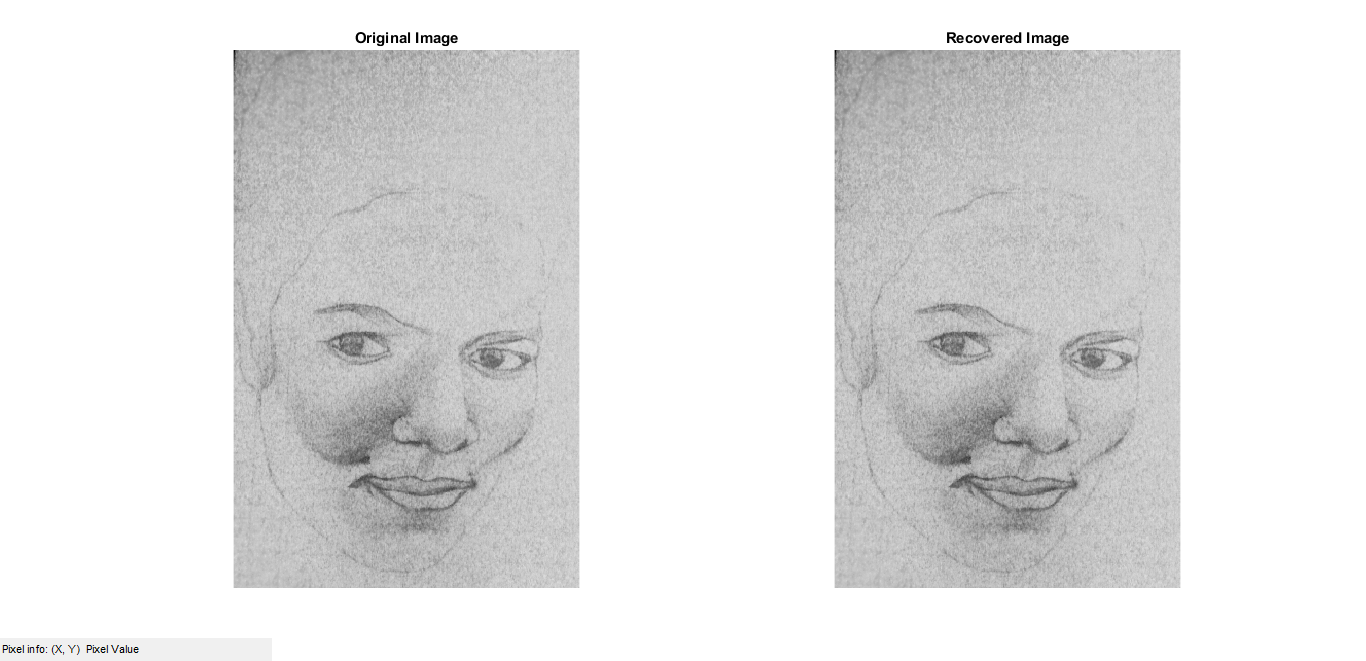
\includegraphics[scale = 0.4]{output_labsix_two.png}\\
\texttt{Figure 2:  Original and Recovered Image from Slicing }\\
For every image operation, the image must be converted to the gray scale image. Then it will be easy for us to apply different filters into that mage as er our requirement.\\
The mean filter gives the image with blurred image. This can be overcome by the use of weighted filter.\\
The salt and pepper noise is added to the image to make it look old or make some dots in the image using the function\\
$\rhd$ \quad imfilter(grayimage, 'salt and pepper', amount\_of\_ noise);\\
The noise is more reduced when we apply the weighted filter that that of the mean filter.\\
This applies same to the gaussian noise. The weighted filter gives clear result than that of using the built-in gaussian filter\\ 
$\rhd$ \quad sigma =3;\\
$\rhd$ \quad cutoff = ceil(3*sigma); \\
$\rhd$  \quad gaussf = fspecial('gaussian', 2*cutoff+1, sigma);\\
$\rhd$  \quad gresult2 = imfilter(g, gaussf); \\
The surface plot of different filters are obtained using the MATLAB function\\
$\rhd$ \quad freqz2(meanf); title('Mean Filter response'); \\
$\rhd$ \quad mf = medfilt2(g,[3,3]);\\
$\rhd$ \quad figure; freqz2(mf); title('Median Filter response'); 
\newpage
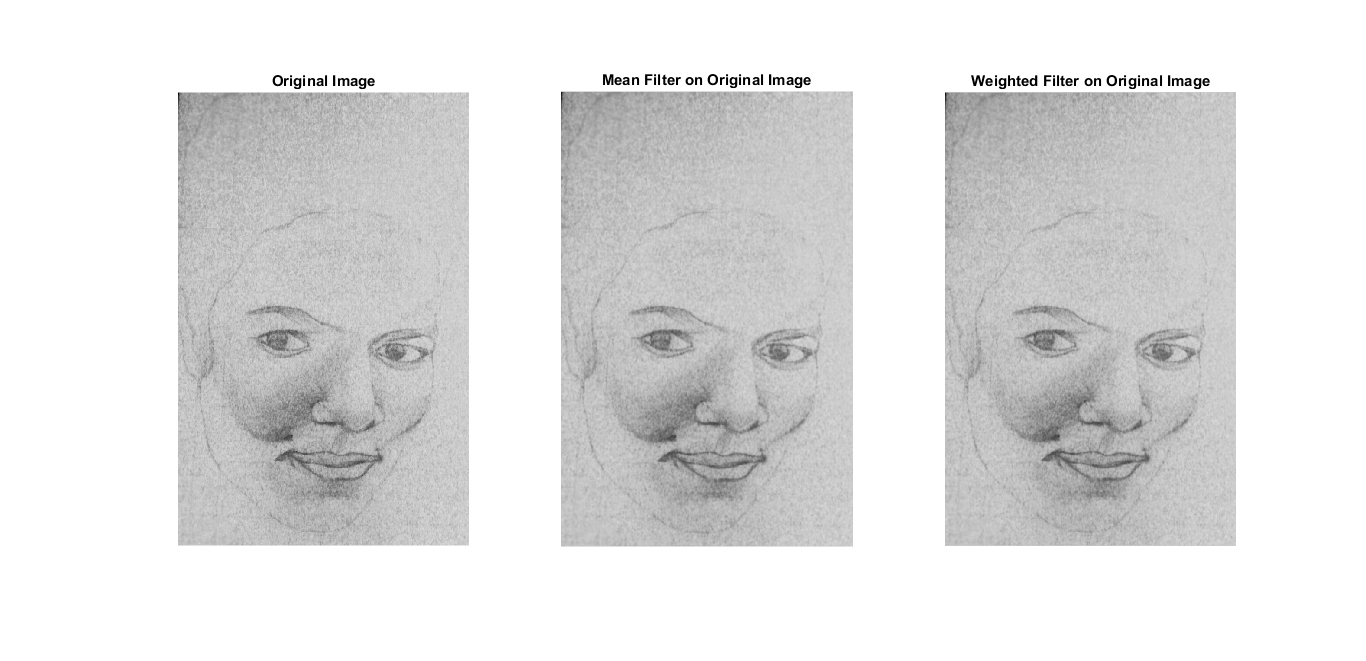
\includegraphics[scale = 0.5]{output_labsix_1.png}\\
\texttt{Figure 3:  Mean and Weighted Filter}\\
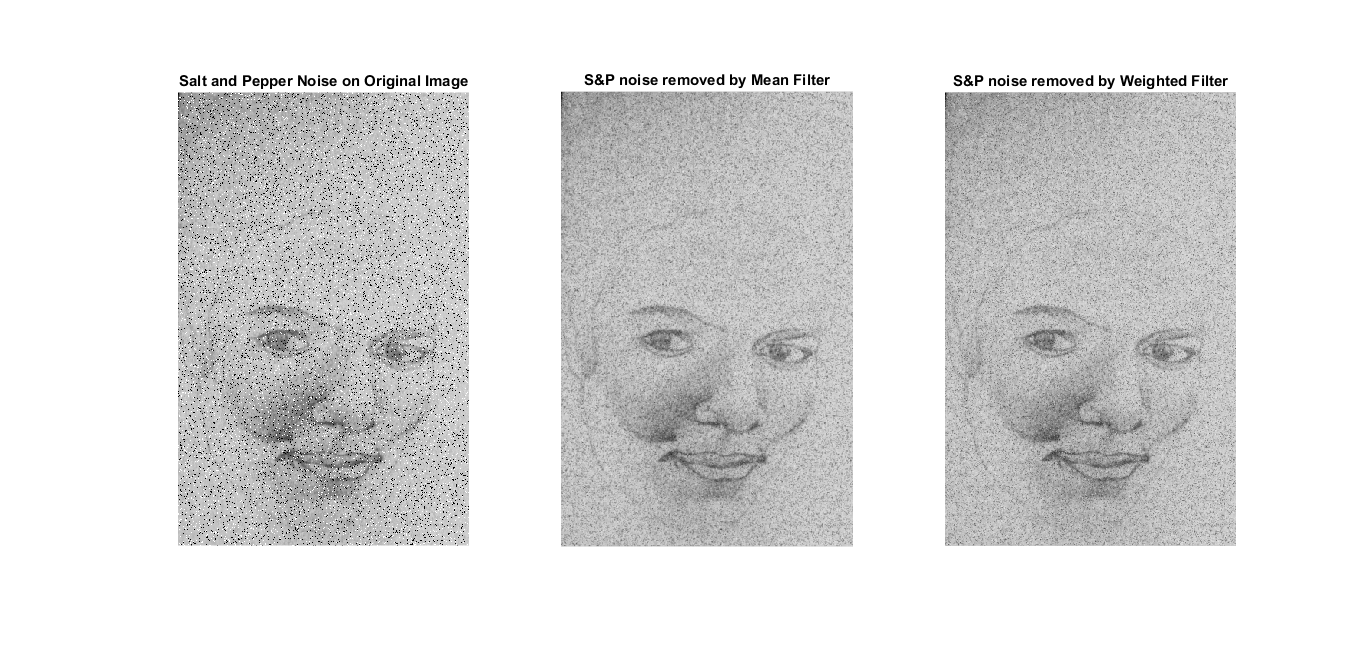
\includegraphics[scale = 0.5]{output_labsix_2.png}\\
\texttt{Figure 4:  Salt and Pepper Noise}\\
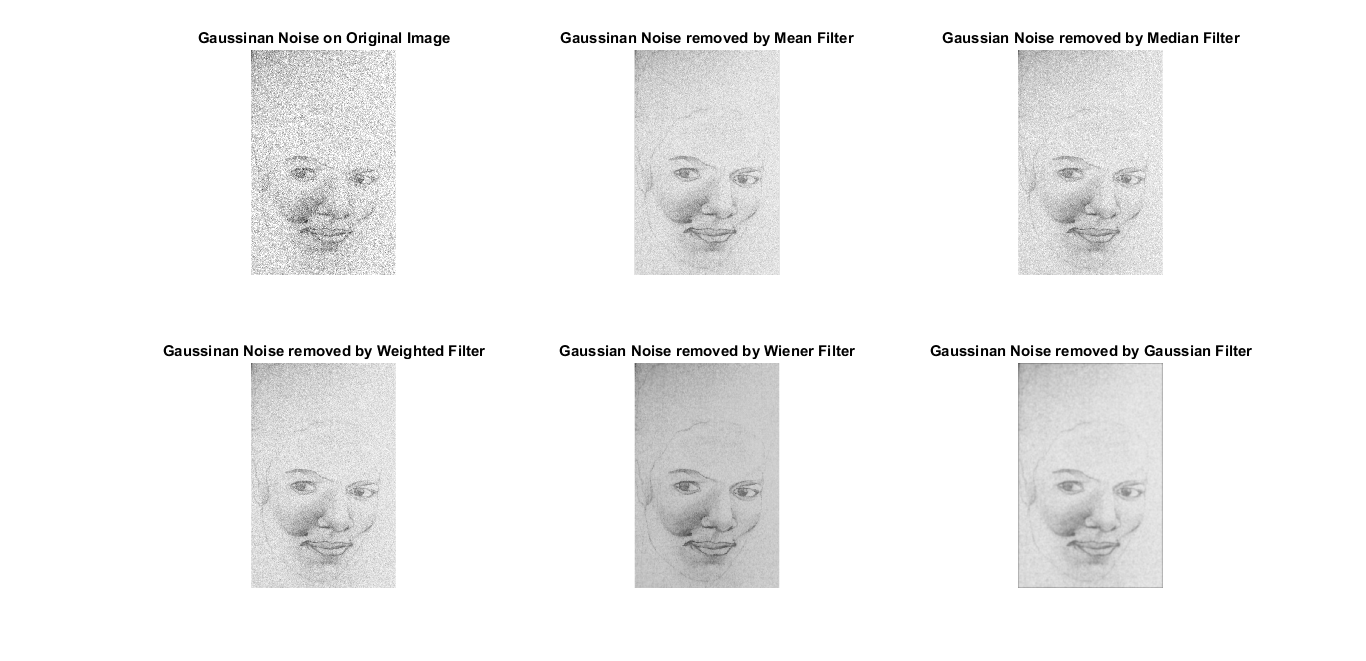
\includegraphics[scale = 0.5]{output_labsix_3.png}\\
\texttt{Figure 5:  Gaussian Noise}\\
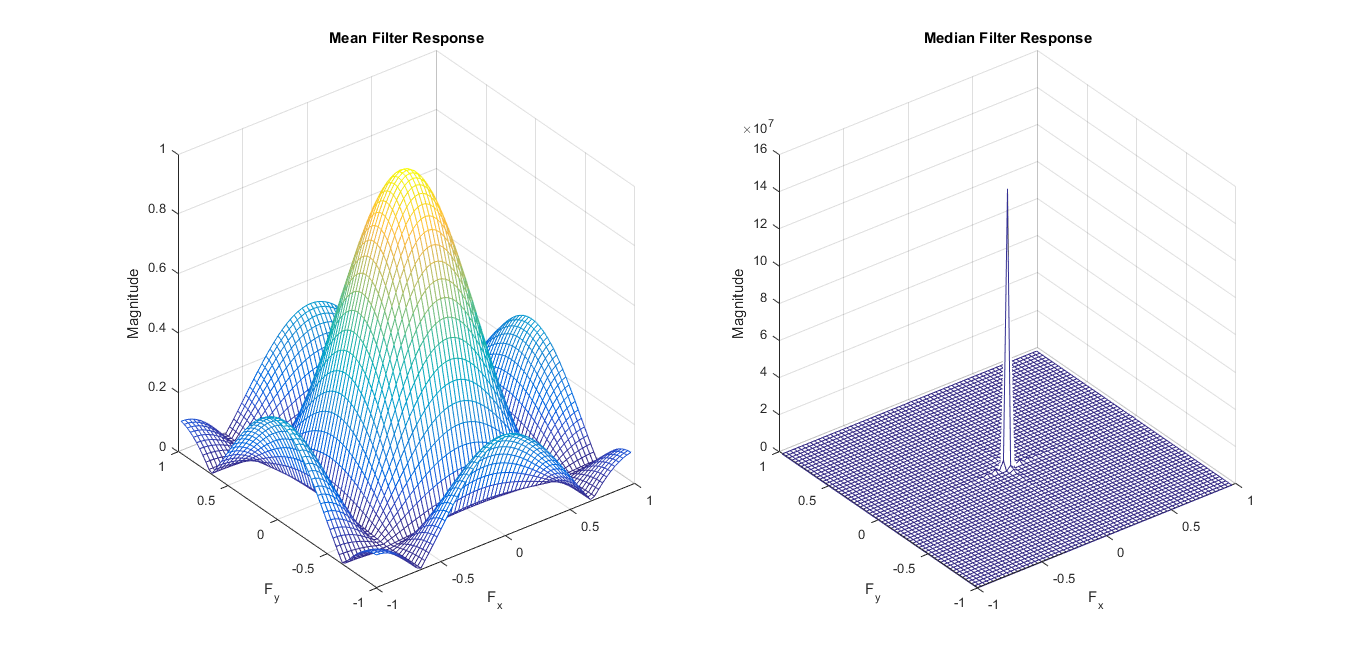
\includegraphics[scale = 0.5]{output_labsix_4.png}\\
\texttt{Figure 6:  Plot of Mean and Median Filter Response}\\

\pagebreak
\section{Conclusion}
Hence, \\
We are familiarized with how the bit plane slicing works and various types of filters, its properties and effects on various types of noises of an image using the MATLAB application.
\end{document}